\documentclass{article}
\usepackage{graphicx}
\usepackage{amsmath}
\graphicspath{ {files/RCP_diagram/} {files/}}

\title{Multi-Scale Resolution of Human Social Systems:  A Synergistic Paradigm for Simulating Minds and Society}
\author{Mark G. Orr}

\begin{document}
\maketitle

\section{Introduction}
Recently, we put forth an Initial sketch of what we call the \textit{Resolution Thesis}\cite{orr2018_brims}.  The thesis holds that 1) models of cognition will be improved given constraints from the structure and dynamics of the social systems in which they are supposed to be embedded, and 2) the resolution of social simulations of agents will be improved given constraints from cognitive first principles\footnote{Cognition considered as theoretical models of human perception, thought and action that includes, broadly, explanations of emotion, motivation, and affect in addition to more tradtional domains of cognitive psychology and cognitive science; one could arguably use the term \textit{psychological first principles} as equivalent}.  This thesis reflects a variety of motivations, the most obvious being the observation that there is little overlap between the cognitive sciences and the generative social science approach, both of which rely heavily on computer simulation to understand aspects of human systems, albeit different aspects of human systems with respect to scale.  The former focuses almost exclusively on the mind as a scientific object of study for which the lion's share of simulation efforts reflect methods that represent a generalizable conception and the latter emphasizes multiple aspects of social systems, the mind being only one of these aspects.  For this latter case,  there is little relation to the vast experimental evidence of how the mind operates or what are the central theoretical entities that compose the mind.  To a large degree, the resolution thesis is a recognition that an interdependence between cognitive science and generative social science has yet to be leveraged for the purposes of improving our understanding of both.    

The Resolution Thesis can be understood from multiple perspectives.  From the generative social science perspective, the Resolution Thesis means that the representations of agents in social simulations should be informed closely by cognitive science and relevant neurophysiological considerations.  This runs somewhat counter to the principled adherence to simplification of the internal processing of simulated agents found in this literature, one that, in fact, served to show that complex social dynamics can be driven by simple behavioral rules of agents.  However, more recently, there are efforts in the generative social sciences that acknowledged that closer ties to the psychological and neurophysiological underpinnings of human behavior may yield benefit.  Epstein's neurocognitive approach is a notable effort in this vein[REF, Epstein 2014]; there are other related approaches (e.g. REF 19-22 from BRiMS).  These efforts notwithstanding, there remains a large gap between them and the implementation of models from cognitive science and psychology, not necessarily in principle, but in practice. It is worth noting that there are some threads in cognitive science that align with this perspective of the \textit{Resolution Thesis}.  In particular, Ron Sun's push for multi-agent systems based on cognitive agents and using cogitive first principles as the basis for the social sciences\cite{sun2006}; other work in this vein exists\cite{Bhattacharyya2010}.  The relatively new field of computational social psychology is clearly relevant\cite{vallacher2017} as well as the computational organizational theory approach\cite{prietula1998}.


From the view of cognitive science, the thesis means that patterns of organization (e.g., information flow on the internet, clustering of behaviors in a community) at the social and organizational level should inform cognitive models when appropriate\footnote{The appropriateness may not be easily determined; for social cognition it may be obvious, but for perceptual domains, e.g., visual categorization, it is not obvious but also highly possible \cite{Culture&Categorization}}.  In other words, these patterns should be included as convergent evidence for a theory or model of cognition.  At first consideration this notion may seem hard to fathom because the implications of cognition for the structure and dynamics of social systems are little understood from the cognitive science perspective\footnote{Anderson's Relevance Thesis, a rare exception, reasons about how cognition may have implications for social organization.}.  Without an explanatory scheme that links facets of the cognitive model to aspects of social organization, how do we interpret the convergent evidence from social systems?  The work mentioned above w.r.t. the cognitive first principles within the generative social science approach \cite{sun2006,prietula1998,vallacher2017,Bhattacharyya2010} begins to put in  place a better understanding of the implications of cognition on social systems, but it is nascent.  

A third and more general view is that the Resolution Thesis is about human social systems.  An understanding of any of these levels of scale is dependent, to some degree, on an understanding of the others.  In effect, the notion of convergent evidence as originating, in part, from other levels of scale, applies to all levels of scale.  The implication is that we should leverage information across scale in an iterative and synergistic way, if not simultaneously. 

The Resolution Thesis, despite sounding somewhat reasonable and practical at face value, is opposed to, some degree, from both the cognitive science and generative social science perspective.  Simon's notion of nearly decomposable systems--that the temporal dynamics of adjacent levels of scale, in most systems, are little correlated--suggests that we can understand well the dynamics at each level of scale independently of the others(*REF, SIM 1962; see P. Anderson, 1972, for similiar argument in phyical systems).  The KISS principle (keep it simple, stupid) used heavily in the generative social sciences, is clearly akin to Simon's notion, and is bolstered by its early wins in understanding the behavior of social systems using simple, non-cognitive agents (REF 15-17 from BRIMS).  In cognitive science, Newell, in considering the time scale of human behavior, suggested that the social band ($> 10^4$ seconds, representing social systems and organizational behavior) is characterized to be weak in strength in the sense that it may not provide computations in a systematic way (relative to lower temporal bands, e.g., cognitive and neural processes).  

These counter arguments notwithstanding, our working assumption is that the degree to which the  \textit{Resolution Thesis} is useful is an empirical issue.  The state of the art in technology, computing and the their tight coupling to the current social mileau affords, we think, the testing of the Resolution Thesis.   To this end, we've developed the \textit{Reciprocal Constraints Paradigm} (henceforth \textit{RCP}), a methodological approach that might lay a foundation for social simulation that is truly multi-scale in nature. 

\section{The Reciprocal Constraints Paradigm}
The value of the \textit{RCP} does not lie in precise formal presecription, but in providing a scaffold for building understanding of social systems, and, possibly providing a deep understanding of the interdependencies among levels of scale.  

\begin{figure}
	\centering
	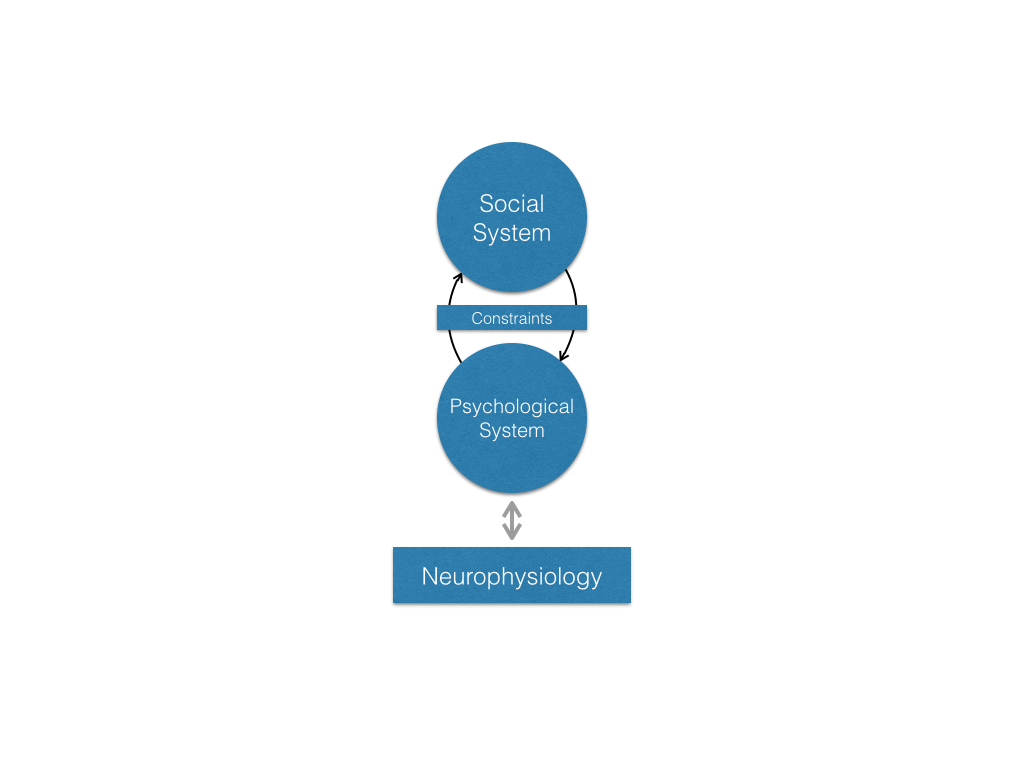
\includegraphics[width=1.0\textwidth]{RCP_diagram.png}
	\caption{\label{fig:rcpdiagram} The four components of the \textit{RCP} are a cognitive system with potential ties to neurophysiology, a social system, and the constraints on each one from the other.  In the \textit{RCP} social systems and cognitive systems are assumed to be derived from and exhibit an abstract set of first principles \& properties, called $S$ and $C$, respectively.  Also captured here is the potential for integrating neurophysiolgical considerations into the cognitive system when appropriate; these may prove as essential for some social systems (the grey two-headed arrow indicates this potential). The notion of constraint refers to the use of information from $S$ \& $C$ to inform one another in a principled way.  
	}
\end{figure}

Figure \ref{fig:rcpdiagram} shows the four primary components of the \textit{RCP}: a cognitive system with potential ties to neurophysiology, a social system, and the constraints between levels of scale.  We assume that social systems and cognitive systems are derived from and exhibit an abstract set of first principles \& properties, called $S$ and $C$, respectively (e.g., theoretial entities, experimental paradigms, patterns in empirical data in respect to the discipines that address a particular level of scale).  Defining $S$ and $C$ will depend on the social system or cognitive system of interest.  The notion of constraint simply refers to the use of information from $S$ \& $C$ to inform one another in a principled way. An upward-constraint refers to information from $C$ informing $S$; downward-constraints reverse this relation.

A primary example in $C$ is the set of allowable algorithms $A$ such that $a \in C$. That is, $A$ defines algorithms that are grounded in and thus recognized by work in cognitive science and psychology.  Primary examples in $S$ are the social structures, channels of information, and dynamic aggregate signals of behavior (e.g., a distribution of degree in a social network over time) that characterize a social system, a large fraction of which is formalized using graph theory/network science.    It is important to emphasize that within $S$ are notions regarding the behavior of agents, not only social structures.

A central assumption in the RCP is that cognitive systems and definitions of agent behaviors in social systems are meant to represent human information-processing capacities that can be described as mathematical functions. \cite{van Rooij, 2008}\footnote{This is equivalent to Marr's computational level; we will use Marr's computational, algorithmic, and implementation levels of description\cite{Marr,1981} throughout this paper.}. Thus, in $C$ we can define a cognitive system as $\psi_{ct}: I_{ct} \rightarrow \psi_{ct}(i)$ where $I_{ct}$ is the set of allowable inputs and $\psi_{ct}(i)$ is the output; in $S$ we have a corresponding agent definition as $\phi_{at}: I_{at} \rightarrow \phi_{at}(i)$ where $I_{at}$ is the set of allowable inputs and $\phi_{at}(i)$ is the output for an agent\footnote{Social and cognitive systems may define parameters regarding variability among a set of agents; this is not reflected here.}. 

\subsection{Applying the Reciprocal Constraints Paradigm}   
In practice there are multiple approaches available for application of the RCT, but what unites them is the study of a human social phenomena, either defined at one level of scale or at multiple levels of scale.  Naturally, the first step is to identify a social phenomena of interest, a task that is inherently tied to one's perspective.  If the perspective is largely cognitive, then the focus would most likely be on understanding the psychological processes, representations, etc. in relation to social systems, but informed in some way by $S$.   Another perspective, at the social scale, would dictate a concern with the social structures and dynamics of the social system (multiple humans interacting) with some degree of constraint from cognitive first principles.  These two perspectives are both what we call single-scale approaches to the \textit{RCP}. Of course, one could take a multi-scale perspective that draws from both and likely depends on a simulation approach that captures aspects of $C$ and $S$ in one runnable system.  

We will address the obvious issues and difficulties in applying the \textit{RCP} after providing a description of some potential methods for application.  The goal in this section is simply to express what it might look like to apply the \textit{RCP}.  

\subsubsection{Single-Scale Approaches}
The single-scale approach of the \textit{RCP} aims to elucidate or refine a model at one level of scale by using some information from another level.  The essence of this approach is captured by the following question: what are the implications of some information from another level of scale for the scale of interest. 
 
Consider the cognitive scale. The single-scale approach amounts to mapping some properties of social systems to properties of cognitive systems for the purpose of identifying potential implications of social structure and dynamics for cognition.  For example, a central finding in cognitive science and psychology is that the products of learning mechanisms are sensitive to the order in which information is presented to the system (e.g., a human's generation of a mental representation of a set of stimuli depends on the order of exposure to the stimuli\footnote{need explanation of this with an example reference}).  The application of the RCT, in this case, means inferring how social features may systematically affect the temporal ordering of stimuli for human contexts. (This seems, almost axiomatically, dependent upon some properties of $S$ if $S$ contains graph $G$ where $V(G)$ and $E(G)$ are the agents and information channels, respectively.).  This is one example of trying to understand the implications of social properties on cognitive systems; what this means precisely would depend on the social phenomena of interest (e.g., early language development may depend on a different $G \in S$ compared to racial stereotypes or large-scale population biases in attitudes).  

At the social level of scale there is a similar approach--mapping the properties of cognitive systems to social systems to reveal potential implications from the former to the latter.  An obvious approach is an analysis of the degree to which $\phi_{at}$ compares to any $\psi_{ct} \in C$ for the purpose of clarifying to what degree a social agent seems to be aligned with cognitive first principles--i.e., what are the implications of cognition for the social system).  For the case in which $\phi_{at}$ and $\psi_{ct}$ are formally well defined, this might be relatively straightforward\footnote{Potential methods for such a comparison would, ideally, focus not only comparison of input/output functions but also the nature of the runnable algorithm}, but this is in no way guaranteed.  There will certainly be cases for which $\psi_{ct}$ is not formally defined\footnote{Many theoretical entities in psychology are not formalized in precise mathematical or computational terms.}.  

A likely scenario is that the closest $\psi_{ct}$ is only defined in terms of an experimental paradigm, ill-defined (non-formal) theoretical definitions and the interpretation of data resulting from application of the experimental paradigm.  So, how does one go about making the comparison when the nature of the two are vastly different?  One approach for comparison for this kind of case would be to explore the behavior of $\phi_{at}$ by simulating an experimental paradigm that is isomorphic to that used to define $\psi_{ct}$ (assuming $\phi_{at}$ is defined algorithmically).  In essence, this is like running an psychological experiment on artificial agents, an approach that is akin to simulation in the psychological sciences.  The output of these experiments could be compared to the patterning and dynamics of human performance in $C$.  This is one suggestion of many potentials, but we hope it illustrates well the potential difficulties.  

%Threshold models of the diffusion of behavior (broadly defined\footnote{The notion of a threshold as a basic agent-level mechanism for social influence spans multiple disciplines from sociology, psychology, demography, and multiple formalisms, e.g., statistical estimation from human data, theoretical treatments from statisitcal physics; In short, it is a broad field } to include theoretical information cascades, voter models, empirical models of human behavior on networks and the diffusion of innovation. NOTE: If we do decide to expand on this approach, then consider asking the question of what cognitive mechanisms would be implicated in standard threshold model behavior, memory, similarity matching, represntation of what? decay, learning, decision methods, reinforcement? 
  
In summary, although the single-scale approach does not represent the full-blown resolution thesis, it might afford better resolution of a target level of scale by considering some of the implications of other levels of scale. The specific phenomena of interest will drive the precise approaches used.

 \subsubsection{Multi-Scale Approaches}
The multi-scale approach is simple in principle: build a simulation platform that simultaneosly captures essential aspects of both $S$ and $C$ (e.g., an agent-based model of cognitive agents).  The upward-constraints would mean a type of substitution of $\psi_{ct}$ for $\phi_{at}$ (substitution might be one approach; for others this might be more akin to a focus or commitment to $\psi_{ct}$). The downward-constraints, generated by some measure of how well the simulated social system matches $S$ as defined by the phenomena of interest, would serve as a signal that would suggest modifications to $S$, $C$ or both.  If this scheme seems simplistic, the details of application are not.

The initial issue is, naturally, to decide where to begin?  Does one start with $S$ and import aspects of $C$ or the reverse?  One might also consider starting from scratch and bringing together properties from $S$ and $C$ in a new way. Let's explore these options via a concrete example which will, we hope, surface some of the key difficulties.  

Imagine we're interested in the patterning of obesity by race/ethnicity, a phenomena of interest with key social and policy aspects (e.g., cultural attractors, social and shared-enviromental influence, spatial patterning co-occuring with racial segregation and residential mobility) and, in fact, a pre-existing set of social simulations from which to draw[REF review paper on simulation of obesity].  Assume we adopt one of the existing simulation approaches, none of which incorporate much in $C$.  Given this case, one approach would be to substitute $\psi_{ct}$ for $\phi_{at}$ while keeping the other aspects identical to the original simulation. In other words, we would be infusing cognition into the agents, so to speak.  

To do this, however, because both $\psi_{ct}$ for $\phi_{at}$ are input-output functions, there is a minimum requirement to find a reasonable substitution such that both $I_{ct}$ and $\psi_{ct}(i)$ are equivalent to both $I_{at}$ and $\phi_{at}(i)$; otherwise, the simulation will not run.  This is non-trivial in the sense that there is a limited but variable set of candidate $\psi_{ct}$ to consider, some or none of which might closely resemble $\phi_{at}$.  The field of obesity in the health behavior tradition has several candidates, each reasonably considered as different (e.g., \{$\psi_{ct_i}, \psi_{ct_j}, \psi_{ct_k},...$\}).  This analysis may be difficult or may limit the degree to which aspects of $\phi_{at}$ can be captured by substitution.  

We are now, already, at an interesting point in this hypothetical scenario because it yields potentially difficult decision points.  For example,  if $\phi_{at}$ does not match any existing $\psi_{ct_i}$, what is implied?  Well, it depends.  At first glance, it seems reasonable to assume that $\phi_{at}$ might be wrong in that it isn't capturing the right set of components.  But, it could be equally true that the health behavior field, in respect to the processes for which the agent model was developed to study, has yet to develop interest in a match for $\phi_{at}$.  One could easily complicate this decision point further or add layers of complication, but we wanted to point out that it gets complicated, fast.  

Let us assume that we find a suitable $\psi_{ct}$ to substitute for $\phi_{at}$. Our next task would be to consider the downward-constraints in this scenario.  Imagine that along with a pre-existing social simulation from which to co-opt, come empirical data, judged of adequate quality, that could be used to compute an objective function w.r.t. the simulations accuracy given our substitution of $\psi$ for $\phi$. This signal, then, would serve as the downward-constraint; i.e., a signal that may indicate issues with the cognitive model\footnote{One might reasonable use the difference between accuracy given $\psi$ and $\phi$ instead for comparison purposes}.  

Let us assume that the simulation does poorly in terms of accuracy; what is to be done?  One might conduct a set of Monte-Carlo simulations to measure the departure from accuracy with respect to the parameters of $\psi_{ct}$ and consider optimizing these parameters to maximize accuracy. But, this raises a serious concern; some would rightly argue that not all parameters in $\psi_{ct}$ should be free to vary on theoretical grounds\cite{Lebiere's accountable modeling Paper}. So, there are theoretical considerations in $C$ that are not directly represented in $\psi$. Another concern is that unless the properties in $S$ captured in the simulation completely reproduce the empirical data (within a reasonable degree of tolerance), one needs to consider, given the objective function, whether to vary some components in the simulation that represent something in $S$.  In other words, in the above scenario it may not be sufficient to only focus on changing $C$; decisions must be made in this regard.   

The above scenario is but one approach, one that is largely \textit{fixing $S$ and importing $C$}.  But what if we \textit{fix $C$ and generate $S$} instead?  What does this look like?  We will stay with the obesity example from above, but change the scenario such that we don't know about any simulation approaches that represent mainly $S$.  Instead, imagine that $S$ is composed of a set of population-level empirical studies, some of which include information on social networks and the built environment, and some theoretcial statements about peer-influence on social networks. Furthermore, similiar to the scenario above, there is a limited set of candidate $\psi_{ct}$ to consider (\{$\psi_{ct_i}, \psi_{ct_j}, \psi_{ct_k},...$\}) in the health behavior tradition and, likely, other aspects of $C$ that may not be represented in them (e.g., categorization, learning, and attractor dynamics).  Further, only one of these candidates\footnote{There do exist a small handful of computationally implemented health behavior theories, see\cite{orr2017readbook; orr2017galeabook} for a review}, $\psi_{ct_i}$, is in a computational formalism; we decide that this will be our starting point.  Analysis of $\psi_{ct_i}$ reveals that it captures the learning and on-the-fly formation of attitudes towards specific health behaviors (considered a precursor to behavior); it is composed in a general manner such that it applies to virtually any health behavior, and; it is empirically grounded using traditional health behavior theory measurment techniques (in one particular behavioral domain). 

These features are useful, but some key components are missing that are akin to first principles of sociological theory.  In particular, $\psi_{ct}$ is mute with respect to the generation of social structure and related dynamics (e.g., decision making for initiating/dissolving relationships; social influence mechanisms in terms of how others' behavior or attitudes can potentially serve as the input to the system).  Thus, at minimum, some decision points arise in terms of how the simulation implements generation and change in network structure the mechanism of social influence.  

To this ends, one could start by implementing a static network topology that captures regularities found in empirical studies of human social networks and disallow change in the network ties as the simulation progresses.  In terms of social influence, we might assume that what is spreading are attitudes and that exposure to others' attitudes can serve as input to an agent and, further there is a knowable stochastic function between attitude and behaviors relating to obesity, e.g., energy balance behaviors relating to caloric intake and use). (As an aside, we've implemented models of this sort \cite{orr2017readbook orr2017galeabook}.)  At this point, we could build out further the social structure and dynamics in relation to the problem of interest using both theoretic and empirical components from $S$, e.g. racial/ethnic distributions in obesity.  

Notice, that what is going on here is a process of building from a cognitive kernel and adding layers of assumptions from $S$ where $S$ includes different kinds of information/footnote{This is very similar to standard practice in social simulation that uses agent-based approaches except that the kernel starts from first principles of computational social psychology.}  At some point, we need to run the simulation and determine how to apply the downward-constraint. We explore this next.

Once the simulation is runnable, the downward-constraint could operate, as describe above, by computing an objective function w.r.t. the accuracy of the simulation compared to extant empirical data.  Here, the issues are mainly the same as in the \textit{fixing $S$ and importing $C$ case described above.}, with an important, subtle difference.  In this case, although, depending on the quality and provenance of the data sources (to mean, roughly, which level of scale do they originate from), there will be decision points in terms of whether to modify $C$ or $S$, the focus should, at least initially, be on $C$.  In the limiting case, imagine that the only data we have is from $C$, e.g., some behavioral studies that reveal something about the learning and formation of attitudes about obesity related behaviors and the relation between attitudes and the behaviors.  All of these studies, further, were conducted at the individual-level and reveal little about social structure and dynamics.  In this case, the objective function would be computed with respect to how well $\psi_{ct_i}$ captures the variation in these data alone.  In this case, it is possible that aspect of both $C$ and $S$ could be modified in the simulation to optimize the objective function.  What is interesting about this limiting case is that $C$ may still depend on $S$.  Getting the $S$ right would be essential.    

These two examples are largely hypothetical.  The value, we hope, is to provide some sketches of what the \textit{RCP} might look like in practice.  Clearly, there are many issues that are raised, even by these sketches, let alone by the general notion of the \textit{RCP} and the \textit{Resolution Thesis}.  We address some of the obvious of these issues next.



  

%\section{An Example of RCT Implemented}
%We now offer an examle of a multi-scale approach to the \textit{RCP}.  It is a highly stylized example that focues much on $C$ using the cognitive architecture ACT-R with some properties of a specific social domain, online social coding in GitHub.  In particular, [describe simulation sketch here]. 

%It will be useful to introduce ACT-R before continuing to the simulations.  ACT-R is a specific approach to modeling human cognition that invokes the idea of a cognitive architecture, a computational instantiation of the structures, mechanisms and represenations of the mind that are coherent with respect to another notion, that of a unified theory of cogntion\cite{newell1990}. A cognitive model that is developed using a cognitive architecture has a potential a constrains operations (if you will it constraints $\psi_{ct}$ to limits of the human mind w.r.t. a unified theory of cognition standpoint.  Cognitive models based on architectures are structured algorithms of $\psi_{ct}$, and, thus, not strictly normative; individual differences are captured naturally in cognitive architectures (e.g., working memory; expertise via domain knowledge).  The generation of quantitative predictions given hypothetical situational domains provides rigor in estimating the quality of model in terms of empirical data.

%ACT-R is composed of several dedicated modules(e.g., procedural and declarative memory, working memory, percetipn and action) that operate in parallel but asychronously vai capacity-limited buffer interfaces.  Each module is composed of independent mechanisms, to include symbolic information processing structures that are combined with equations for the representation f specific regularities and phenomena (e.g., reinforcement learning, power law of practice, power law of forgetting).  Further, ACT-R adapts to environmental structure via a number of learning mechanisms.  In short, it provides an account of human informaion processing capability and limitations (e.g., inherent biases) precicely because of the coupling of computational mechanisms and limits on capacity (e.g., working memory, attention).   

%Using a cognitive architecture, versus any cognitive model, characterizes well what agents are supposed to do in the generative social science approach--adaptive behaviors that are coupled to the social and physical environment.  ACT-R, in particular, has modeled a broad range of human behaviors to include language, complex decision making, experimental psychology paradigms, and dynamic task environments (see the ACT-R web site\cite{ACTRWEBSITE}).  Of particular relevance for this paper are some efforts using ACT-R as the basis for agents in multi-agent social simulations--e.g, iterated two-player games, bot adversarial and cooperative \cite{hi}

%\subsection{Importing Neurophysiology}
%Base this on Stocco's paragraph from BRiMs and use it in the context of the ACT-R sim we did above. and 

%Also, add the paragraph from BRiMS on how neuro to cog is many to one and cog to social is one to one.


\section{Discussion}
The RCP as described above, with the single and multi-scale approaches attempted to illustrate some of the ways that it might be implemented now.  However, to our mind, this is only useful to motivate the development of a more systematic body of work and approach that is moving towards the goals of the Resolution Thesis.  Now we want to look forward and think about the next generation of the RCP. But first, let us point out some of the 

\subsection{Issues in Applying the Reciprocal Constraints Paradigm }
Both single- and multi-scale approaches to the \textit{RCP} are fraught with difficulty in application.  

2. FREE PARAMETER PROBLEM AND Acountable modeling, mere parameter optimization?: 


4. Many competing cog models for any phenomena ... Issues of the right cogntive model, lots of cog models....

5. Downward constraints in multi-scale approach....what precisly is changed

6. quality of the data...some are quite veridical on some dimensions, but may be misleading on others...e.g., tweets are tmeporal and veridical in terms of content, but inference about meaning, motivation and intention may not be possible.  data issues in general...the case when there is little data or there is a patchwork of data.



The second kind is to abstract some details from full-fledged cognitive models, but adhere to a principle of \textit{Accountable Modeling}\ref{LebiereX}.

Have data at both levels or just one...re

\subsection{Moving Forward}
From the single level of scale approach, One idea is to catalog social phenomena captured by psychological models and do a mapping of $C$ to $S$. \footnote{In the limit, the social features and the cognitive features have co-evolved on an evolutionary time scale}.

Downward constraints on neurophysiology? From neuro to cog to social to cog to neuro?  Is this where it is headed? Stocco has a paragraph in BRiMS on the cog to neuro, use it.

A modular, iterative appraoch:  It may be apparent to the reader that the multi-scale approach to the RCP, given the current state of the art, is somewhat piecemeal.  One is forced to coble together a shoe from parts of kitchen objects...Not impossible, but not optimal.  So, in closing, we would like to suggest the following idea.  What is needed is a modular, iterative approach that begins to build social structure from first principles of lower levels of scale.  



  




\bibliographystyle{plain}
\bibliography{references}

\end{document}